\chapter{模态逻辑,知识的逻辑}\label{chap:modal-logic}

你听说过魔芋与高僧的故事吗?相传,这个有趣的故事发生在日本的一座深山之中。在那幽静的山谷中,有一座古老而荒废的寺庙,几百年来一直无人问津,只有密林与野兽相伴。

一天,一个以卖魔芋为生的流浪小贩推着他的木车,偶然来到这片偏僻的地方。他发现这座破旧的寺庙中竟然无人居住,便心想:“如此偏僻之地,不如就在此地安顿下来吧。”于是,他便住了下来,每天挑着魔芋,走村串户,卖给山中偶尔路过的行人。

不久之后,一位云游四方的僧人也来到了这片深山。看到这座荒废的寺庙,他心生好奇,便前去查看。僧人惊讶地发现寺庙中竟然住着一位老人,便以为这是位得道高僧。僧人心中一动,想着既然能在如此偏远之地修行,必定有过人之处,于是便恭敬地上前,请教佛法。

在佛教传统中,有一种不动声色的辩经方式,那就是只用手势来比划,而不发一言。僧人遵循这一传统,开始用手势向卖魔芋的人比划起来。然而,卖魔芋的人哪里知道这些佛教传统?他误以为僧人是在挑剔他卖的魔芋不好,来讨说法的。他心中不悦,但还是用手势回应僧人,心想着:“我卖的魔芋可是顶好的,若是敢挑衅,我便和你理论理论!”

于是,两人各怀心事,展开了一场激烈的手势比划。僧人暗自佩服卖魔芋的人的沉稳与深不可测的手势,心想自己在佛法修行上还有很大的差距;而卖魔芋的人则越比越得意,心中大呼:“这人还真有些手段,但我魔芋的品质岂是一般人能质疑的?”

比划结束后,僧人心生敬意,深感不如;卖魔芋的人则自信满满,觉得自己的魔芋赢得了这场对峙。因此,“卖魔芋的人获胜”这件事成了他们二人的共同知识。然而,两人心中所思所想却完全不同!僧人认为自己遇到了高人,而卖魔芋的人则确信自己击退了一个挑刺的顾客。

在\Cref{chap:bayesian-game}中,我们探讨了知识的一些基本性质。上面的魔芋故事实际上揭示了两件重要的事情:
\begin{itemize}
    \item 一方面,知识(尤其是共同知识)要比我们想象的复杂得多。在这个例子中,两个人知道的“事实”究竟是不是同样的呢?这个问题并不容易回答。
    \item 另一方面,知识的传递与理解可以超越自然语言。在这个例子中,两人完全没有用语言交流,而是依靠手势。这说明知识可以有不同于自然语言的表达方式。
\end{itemize}

在本章中,第二点将是我们的讨论重点。它意味着我们可以用形式逻辑来描述知识的概念和性质。这种形式逻辑在现代逻辑学中被归类为\emph{模态逻辑}。模态逻辑是一种扩展了经典形式逻辑(如命题逻辑和一阶逻辑)的逻辑,通过引入\emph{模态词}——例如“必然”、“可能”、“知道”等——来描述命题的性质。最后,作为一个例子,我们将使用模态逻辑的语言表述并证明Robert Aumann的“对不一致达成一致”定理。

\section{知识逻辑的形式语言}

\emph{模态词}是指说话者对语句的限定。不同的限定反映了不同的逻辑状态。例如:\emph{必然}、\emph{可能}、\emph{过去}、\emph{未来}、\emph{知识}、\emph{信念}和\emph{可证明}等,都是典型的模态概念。比如,我们可以说“明天可能会下雨”、“我知道明天会下雨”、“我相信明天会下雨”、“明天可能会下雨”等等,他们要表达的意思并不是经典逻辑可以表述的。

在经典逻辑中,我们只能表达“明天下雨”或者“明天不下雨”这样的命题。因而,\emph{模态逻辑}提供了一套严密的数学工具,可以把模态的概念从自然语言中“搬到”形式语言中。

因为模态词往往都与人的认知和思维有关,因此,通过模态逻辑,我们可以算法化、自动化地模拟和推理人类的思维和认知过程。这正是人工智能中\emph{符号主义}的思想。

在研究模态逻辑时,重要的一部分是研究它的\emph{模型论},即如何定义模态逻辑的语言、然后赋予这些形式语言具体的含义与真假,即\emph{语义}。

模型论的角度看,一个逻辑系统包括三个要素:\emph{语言}、\emph{模型}、\emph{语义}. 他们分别代表,我怎么说话、我关心的对象是什么、我说的话和我关心的东西之间有什么关系。接下来,我们以命题逻辑为例,介绍三要素。

\begin{example}[命题逻辑的逻辑三要素]
命题逻辑是由命题字母、逻辑联结词和括号组成的形式语言。例如,$p\to q$这样的东西属于命题逻辑,但是$\forall x\, P(x)$这样的东西不属于命题逻辑(而属于一阶逻辑)。关于命题逻辑更系统的讨论,请参阅\Cref{chap:plausible-reasoning}。

命题逻辑的三要素是:

\begin{itemize}
    \item 语言(我怎么说话):用规则写成的字符串,例如我们可以用字符串$p\to q$表示一个逻辑公式,但是不能写$\forall x\, P(x)$、$2+2=4$或者$p\vee\vee q$。我们可以简单理解成,我们说普通话的时候,不能说英语,也不能说语法错误的句子(如“我是是”)。
    \item 模型(我们关心的对象是什么):我们关心的世界结构,在命题逻辑中就是“真”和“假”. 因此,在命题逻辑的世界里,没有实数,也没有人类,更没有诗和远方;只有冰冷(但是精确)的“真”和“假”。
    \item 语义(我说的话和我关心的东西之间有什么关系):我们可以先给命题字母真假的概念,例如$p$赋值为“真”,$q$赋值为“假”. 当每一个命题字母都被赋予了真假之后,我们就可以定义整个公式的真假。例如,$p\to q$为真当且仅当$p$为假或者$q$为真。
\end{itemize}
\end{example}

尽管在\Cref{chap:plausible-reasoning}中,我们也简要介绍了逻辑三要素。但是,我们在这里才将这样的讨论展开。这是因为,只有到了模态逻辑的世界,逻辑三要素才变得如此不平凡,我们才能真正体会到他们的意义。接下来,我们将介绍模态逻辑的语言、模型和语义。本节先介绍模态逻辑的语言。

首先,我们只考虑最简单的情况,基础语言是命题逻辑,然后在其中加入一个\emph{模态算子}。

\begin{definition}[基本模态语言]
给定命题字母表$\mathbf P$,我们定义它的\textbf{基本模态语言} $L$,按照如下方式递归生成:
\begin{itemize}
    \item 命题字母$p\in \mathbf P$属于$L$,$\top$属于$L$。
    \item 如果$\phi$属于$L$,那么$\neg\phi$ 和$\Box\phi$也属于$L$。
    \item 如果$\phi_1,\phi_2$属于$L$,那么$(\phi_1\wedge\phi_2)$也属于$L$。
\end{itemize}
\end{definition}

和命题逻辑比较,我们多了一个模态算子$\Box$,它读作“Box”,对应的自然语言可以读为“必然”(更多讨论见本部分后文)。

我们在后面将会频繁定义各种不同的模态语言,为了方便,我们引入一种更简洁的记号:
\[\phi\quad::=\quad p\mid \top\mid \neg\phi\mid (\phi\wedge\phi)\mid \Box\phi.\]
这种记号被称为\emph{Backus-Naur范式}(\emph{BNF}),是一种用来描述形式语言的标准记号,在编程语言设计和编译器的实现中也经常使用。

类似命题逻辑,我们有如下缩写:
\begin{itemize}
    \item $\phi\vee\psi\iff\neg(\neg \phi\wedge\neg\psi)$.
    \item $\phi\to\psi\iff\neg\phi\vee\psi$.
    \item $\bot\iff\neg\top$.
\end{itemize}

引入模态算子$\Box$之后,我们还有它对应的\emph{对偶}算子$\Diamond$,它是如下的缩写:
\[\Diamond\phi\iff\neg\Box\neg\phi.\]
$\Diamond$读作“diamond”,对应的自然语言可以读为“可能”。为什么它的自然语言解释是“可能”呢?因为,“不是必然不”的意思就是“可能”。$\Box$和$\Diamond$的对偶性,我们可以类比$\exists$和$\forall$的对偶性,这是因为$\exists$也可以写成$\neg\forall\neg$。我们将在\Cref{sec:kripke-semantics}中看到,这一类比其实有极其自然的模型论解释。

既然可以加入一个模态算子,我们也可以加入更多的模态算子,一个模态算子也可以修饰多个公式。例如,我们可以引入一个新的模态算子$\Box_a$,表示个体$a$认为的必然性。于是,我们可以写出这样的公式:
\[\Box_a\phi\wedge\Box_b\psi\to\Box_a(\phi\wedge\psi).\]
我们也可以引入模态算子$\nabla(\phi,\psi)$,表示$\phi$成立的时候,$\psi$必然成立。于是,我们可以写出这样的公式:
\[\nabla(\phi\to\psi,\Box\phi)\to\Box\psi.\]

通过引入不同的模态算子来描述不同的对象,模态逻辑被赋予了这样的哲学:多视角下看同一个数学概念。比如,我们可以把$\Box$在自然语言中用不同的词来解释,由此得到不同的模态逻辑:
\begin{itemize}
    \item 基本模态逻辑:可能/必然是
    \item 时序逻辑:将会是
    \item 道义逻辑:被允许是
    \item 知识逻辑:被知道是
    \item 可证性逻辑:可以被证明是
    \item 动态逻辑:(在经过某些程序步骤之后)会是
\end{itemize}

接下来,我们具体看两个例子,这是本节最关心的两种解释:\emph{基本模态逻辑}和\emph{知识逻辑}。
\begin{example}[基本模态逻辑]
我们可以把模态算子$\Box$读成“必然”。于是,
\begin{itemize}
    \item $\Box\phi$ 表示“必然有$\phi$”。
    \item $\Diamond\phi$ 表示“不是必然有非$\phi$”,即“可能有$\phi$”,所以$\Diamond$读作“可能”。
    \item 反之,$\Box\phi$也可以读作“不可能有非$\phi$”,即“必然有$\phi$”。
    \item 因此,$\Diamond$和$\Box$确实是对偶的。
\end{itemize}

在这个读法下,我们可以用形式语言去表达一些自然语言中很拗口的句子,但更加清晰和精确。比如:
\begin{itemize}
    \item $\Box p\to\Diamond p$:必然的事也是可能的。
    \item $p\to\Box p$:真的事是必然的。
    \item $\Diamond p\to\Box\Diamond p$:可能的事是必然可能的。
\end{itemize}
\end{example}

\begin{example}[知识逻辑]

在知识逻辑中,我们可以把模态算子$\Box$读成“知道”,并写成$K$(know)。$K$表示某个特定的个体对世界的认知。例如:

\begin{itemize}
    \item $K\phi$(即$\Box\phi$):我知道$\phi$。
    \item $K\phi\to\phi$:如果我知道$\phi$,那么$\phi$是真的。
    \item $\phi\to K\phi$:如果$\phi$是真的,那么我知道$\phi$。
    \item $\neg K\phi$ vs. $K(\neg\phi)$:我不知道上帝存在 vs. 我知道上帝不存在。这两句话的含义是不同的,因此,模态词使得否定的含义变得复杂。
\end{itemize}

在更一般的情况下,我们会有多个个体,于是可以用$K_a$表示“个体$a$知道”。同样,我们可以用$B_a$表示“个体$a$相信”。这里是一些例子:

\begin{itemize}
    \item $K_aK_b\phi\leftrightarrow K_bK_a\phi$:我知道你知道$\phi$当且仅当你知道我知道$\phi$。
    \item $K_1K_2p\wedge \neg K_2K_1K_2 p$:$1$知道$2$知道$p$,但是$2$并不知道$1$知道$2$知道$p$。
    \item $\neg K_i p\to K_i(\neg K_i p)$:如果我不知道$p$,那么我知道我不知道$p$。
    \item $K_i(p\wedge\neg K_i p)$:我知道如下的陈述:$p$是真的,且我不知道$p$。一种类似的写法是,$K_ip\wedge K_i\neg K_ip$,即我知道$p$,但是我又知道我不知道$p$。
    \item 共同知识算子\footnote{这个算子的定义以及性质在\Cref{sec:epistemic-logic-basic-model}中会详细讨论,这里仅作为一个例子,读者不必理解具体的意义。}$C$:$C \phi$当且仅当$K_a(\phi\wedge C\phi)$对任意$a$成立。注意,$C\phi$并不等价于对任意$a$,$K_a\phi$成立。
\end{itemize}
\end{example}

\section{Kripke语义}\label{sec:kripke-semantics}

接下来我们讨论模态语言对应的模型,以及模态逻辑语言在这一模型上的语义。从本节开始,我们将模态算子限制为\emph{一元}算子,即它只能修饰一个公式。

我们考虑的模型被称为\emph{Kripke(点)模型}。它可以看作是一个带有标记的有向边和节点的图:
\begin{itemize}
\item 节点表示可能世界,上面用命题字母标记,表示这个可能世界上成立的原子命题;
\item 边表示节点之间的关系,用模态算子标记,表示这两个可能世界之间的关系。如果只有一个模态算子,我们省略模态算子标记,只写箭头。
\item 我们有一个指定的节点,作为真实世界。
\end{itemize}

我们来看一个例子。

\begin{example}
我们可以用下面的\Cref{fig:kripke-model-basic} 来表示一个Kripke模型。

\begin{figure}[ht]
\centering
\documentclass{standalone}
% font set
\usepackage{ctex}
\usepackage{fontspec}
\usepackage[T1]{fontenc}
\usepackage[sc]{mathpazo}
\usepackage{anyfontsize}
\setmainfont{Source Serif 4}
\setsansfont{Source Sans 3}
\setmonofont{Menlo}
\setCJKmainfont[BoldFont=黑体-简 中等,ItalicFont=楷体-简 常规体]{宋体-简 常规体}

% colors
\usepackage[dvipsnames]{xcolor}
\definecolor{pku-red}{RGB}{139,0,18}
\usepackage{colortbl}
\newcommand{\light}[1]{\textcolor{Orchid}{#1}}
\newcommand{\contrastlight}[1]{\textcolor{TealBlue}{#1}}

% plots
\usepackage{tikz}
\usepackage{tikz-cd}
\usetikzlibrary{arrows}
\usetikzlibrary{arrows.meta,positioning,calc,3d}

% math package
\let\Bbbk\relax
\usepackage{amsmath}
\usepackage{mathrsfs}
\usepackage{amssymb}
\usepackage{amsfonts}
\usepackage{stmaryrd}
\usepackage{extarrows}
\SetSymbolFont{stmry}{bold}{U}{stmry}{m}{n}


% math notations
\newcommand{\LHS}{\mathrm{LHS}}
\newcommand{\RHS}{\mathrm{RHS}}
\newcommand{\Z}{\mathbb{Z}}
\newcommand{\N}{\mathbb{N}}
\newcommand{\R}{\mathbb{R}}
\newcommand{\Q}{\mathbb{Q}}
\newcommand{\C}{\mathbb{C}}
\newcommand{\E}{\mathbb{E}}
\renewcommand{\O}{\mathcal{O}}
\newcommand{\id}{\mathrm{id}}
\DeclareMathOperator*{\Span}{Span}
\DeclareMathOperator*{\im}{Im}
\DeclareMathOperator*{\rank}{rank}
\DeclareMathOperator*{\card}{card}
\DeclareMathOperator*{\grad}{grad}
\DeclareMathOperator*{\argmax}{argmax}
\DeclareMathOperator*{\epi}{epi}
\DeclareMathOperator*{\maximize}{maximize}
\DeclareMathOperator*{\minimize}{minimize}
\renewcommand{\d}{\mathrm{d}}
\newcommand{\Pow}{\mathcal{P}}
\newcommand{\cov}{\mathsf{Cov}}
\newcommand{\var}{\mathsf{Var}}
\newcommand{\Nor}{\mathcal{N}}
\newcommand{\U}{\mathcal{U}}
\renewcommand{\t}{\mathsf{T}}
\newcommand{\T}{\top}
\newcommand{\F}{\bot}
\newcommand{\norm}[1]{\left\|#1\right\|}
\newcommand{\inner}[2]{\left\langle{#1},{#2}\right\rangle}
\newcommand{\e}{\mathrm{e}}
\newcommand{\const}{\mathrm{const}}
\newcommand{\scB}{\mathscr{B}}
\newcommand{\scF}{\mathscr{F}}
\newcommand{\G}{\mathscr{G}}
\newcommand{\Exp}{\mathsf{Exp}}
\newcommand{\DExp}{\mathsf{DExp}}
\newcommand{\Lap}{\mathsf{Lap}}
\newcommand{\calP}{\mathcal P}
\newcommand{\calS}{\mathcal S}
\newcommand{\calF}{\mathcal F}
\newcommand{\calM}{\mathcal M}
\newcommand{\KL}{\mathrm{KL}}
\newcommand{\ReLU}{\mathsf{ReLU}}
\newcommand{\val}{\mathsf{val}}

\begin{document}
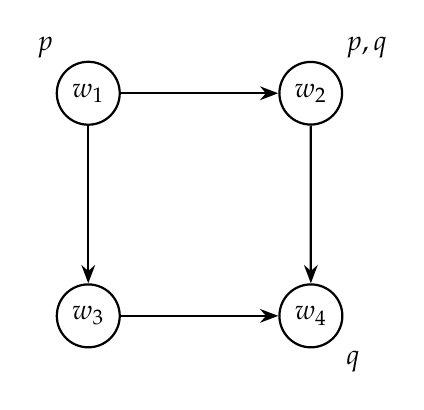
\begin{tikzpicture}[node distance=2cm,thick,>=Stealth]
\node (w1) [circle,draw] {$w_1$};
\node (w2) [circle,draw,right=of w1] {$w_2$};
\node (w3) [circle,draw,below=of w1] {$w_3$};
\node (w4) [circle,draw,right=of w3] {$w_4$};
\draw[->] (w1) -- (w2);
\draw[->] (w1) -- (w3);
\draw[->] (w2) -- (w4);
\draw[->] (w3) -- (w4);
\node [above left=1pt of w1] {$p$};
\node [above right=1pt of w2] {$p,q$};
\node [below left=1pt of w3] {};
\node [below right=1pt of w4] {$q$};
\end{tikzpicture}
\end{document}
\caption{Kripke模型的示例}\label{fig:kripke-model-basic}
\end{figure}

模型中,一共有四个可能世界,用$w_1,w_2,w_3,w_4$表示。他们之间的关系用箭头表示,例如$w_1\to w_2$表示$w_1$到$w_2$有模态算子$\Box$对应的关系。我们可以把箭头更直观地理解为,从$w_1$这个世界的视角看,他能够想象一个$w_2$的可能世界。

我们还要指定一个节点作为真实世界,这里我们指定$w_1$作为真实世界。
\end{example}

我们将节点解读为\emph{可能世界}。此时,$\Box$被理解为“必然”,$\Diamond$被理解为“可能”。接下来,我们把模态的语言和模型联系起来,定义模态逻辑的语义,完成模态逻辑三要素的定义。

设想,在真实世界$w_1$,我们说$\Box p$是真的,换言之,“必然有$p$”。当我们在说这句话的时候,我们其实在脑中想象了所有能想到的可能世界,然后发现在所有可能世界中,$p$都是真的,于是,我们才说,“必然有$p$”。这就是模态逻辑的语义。

形式化地说,$\Box\phi$在世界$w$上成立当且仅当$\phi$在$w$的所有后继上为真。这种语义通常被称为\emph{Kripke语义}或\emph{可能世界语义}。在一个世界讨论可能与必然的时候,会取决于它与其他世界的联系。

我们再来看一个例子。

\begin{example}\label{ex:kripke-model-basic}
考虑\Cref{fig:kripke-model-basic} 中的Kripke模型。对哪些$i$来说,下式成立?
\[\Box (p\to\Box q).\]
我们以$w_1$为例进行讨论。其他情况非常类似,读者可以自行验证。如果$w_1$是真实世界,上要成立上式,必须要所有后继节点上成立
    \[p\to\Box q.\]
$p$的后继节点有$w_2,w_3$,分别考虑这两个节点:
\begin{itemize}
    \item 对于$w_2$,$p$为真,所以需要看$\Box q$是否成立。$w_2$的后继节点只有$w_4$。注意到,$w_4$上$q$为真,因此$w_2$上$\Box q$成立,所以$w_2$上$p\to\Box q$也成立。
    \item 对于$w_3$,$p$为假,所以$p\to\Box q$自动成立。
\end{itemize}
因此,$w_1$上$\Box (p\to\Box q)$成立。同理,我们可以验证其他节点上的情况,得到在$w_2$,$w_3$,$w_4$上,$\Box (p\to\Box q)$都成立。

特别注意,在验证$w_4$的时候,因为$w_4$没有后继节点,所以任何命题$\phi$,$\Box\phi$都是成立的。
\end{example}

游了对概念的自然语言描述和例子,接下来,我们形式上给出模态逻辑的模型和语义定义。

首先,定义一个\emph{Kripke框架},它单纯描述可能世界及其之间的关系,不考虑可能世界上有哪些命题成立。

\begin{definition}[Kripke框架]
考虑基本命题模态逻辑$L$。一个\textbf{Kripke框架}是一个元组$\mathcal F=(W,R)$,其中:
\begin{itemize}
\item $W$是非空集合(可能世界集);
\item $R\subseteq W\times W$是一个$W$上的二元关系(边)。
\end{itemize}
\end{definition}

接下来,对每一个可能世界,我们赋予它为真的原子命题,如此得到了一个\emph{Kripke模型}。

\begin{definition}[Kripke模型]
一个\textbf{Kripke模型}$\mathcal{M}$是一个元组$(\mathcal F,V)$,其中$\mathcal F$是Kripke框架,$V:\mathbf W\to 2^{\mathbf P}$是\textbf{赋值函数},表示每个可能世界上为真的那些命题字母(即原子命题)。
\end{definition}

Kripke模型并没有指定一个真实世界,接下来,我们引入一个指定的点,作为真实世界,得到\emph{Kripke点模型}。

\begin{definition}[Kripke点模型]
一个\textbf{Kripke点模型}$(\mathcal{M},w)$是Kripke模型$\mathcal M$加上一个指定的点$w\in W$。
\end{definition}

现在,我们可以定义模态逻辑的语义,即\emph{Kripke语义}。

\begin{definition}[Kripke语义]
考虑基本命题模态逻辑$L$。符号$\mathcal M,w\vDash\phi$表示$\phi$在点模型$\mathcal M,w$是\textbf{可满足的}。这一概念可以递归定义如下:
\begin{itemize}
\item $\mathcal M, w\vDash\top$永远成立。
\item $\mathcal M, w\vDash p$当且仅当$p\in V(w)$。
\item $\mathcal M, w\vDash (\phi\wedge\psi)$当且仅当$\mathcal M,w\vDash\phi$且$\mathcal M,w\vDash\psi$。
\item $\mathcal M, w\vDash \neg\phi$当且仅当$\mathcal M,w\not\vDash\phi$。
\item $\mathcal M, w\vDash \Box\phi$当且仅当对所有$v$,如果$wRv$,那么$\mathcal M,v\vDash\phi$。
\end{itemize}
因此,$\mathcal M, w\vDash \Diamond\phi$当且仅当存在$v$满足$wRv$且$\mathcal M,v\vDash\phi$。
\end{definition}

注意,上面的定义都是在只有一个模态算子的情况下定义的。不过,我们可以很容易地推广到多个一元模态算子的情况。假设模态算子是$\Box_a$,那么Kripke框架中的边需要附上标签$a$,表明这个边是$\Box_a$对应的关系,即$w\to_a v$。在这种情况下,$\Box_a\phi$的语义定义为:对所有$v$,如果$wR_av$,那么$\mathcal M,v\vDash\phi$。

多个一元模态算子在知识逻辑中是很常见的。每个人都有自己对于世界的认知,因此每个人$a$在模型中会有一个对应的关系$R_a$,以描述他所认为的可能世界架构,$R_a$对应的$\Box$模态算子写作$K_a$。

现在,我们进一步讨论语义的性质。逻辑公式的语义,无论如何定义,其实都在讨论“什么是真的”这一基本问题。在模态逻辑中,这一概念尤其复杂。

比如,在\Cref{ex:kripke-model-basic} 中,我们讨论了$\phi:\Box (p\to\Box q)$在一个Kripke模型中每个可能世界上的真值。在例子的计算中,我们发现,所有可能世界上$\phi$都是真的。所以,我们其实可以说,$\phi$在整个Kripke模型上也是真的。

更进一步,我们也想知道一些关于可能和必然的真理。为了说明这一点,先回到命题逻辑中,考虑任意命题字母$p$,无论$p$是否是真的,下面这个公式永远都是真的:
\[p\to p.\]
我们在命题逻辑中称这样的公式为\emph{重言式}. 重言式其实反映了命题逻辑的一些根本性质,这些性质独立于具体的命题而存在。比如\emph{排中律}:对于任意命题$p$,$p\vee\neg p$是重言式,再比如\emph{三段论}:$((p\to q)\wedge p)\to q$是重言式。他们是我们做逻辑推理的时候自动会假设的性质。

同样的问题也可以对模态逻辑提出:有没有一些关于可能和必然的性质,是独立于具体的可能世界而存在的?比如,我们是否可以说,如果$p$是真的,那么$p$必然是真的?把它写成模态逻辑的形式就是:
\[p\to \Box p.\]
如果这是一个关于必然的真理,那么,无论$p$是否为真,无论我们处于什么样的可能世界,这个公式都应该是真的。

根据上面的启发,在模态逻辑的体系中,我们可以定义各种不同粒度的“真”的概念:

\begin{definition}[模态逻辑的真值]
给定模态逻辑公式$\phi$,我们可以定义它的真值:
\begin{itemize}
\item $\phi$在点模型$\mathcal M,w$\emph{可满足}指的是$\mathcal M,w\vDash \phi$。
\item $\phi$在模型$\mathcal M$\emph{有效},记为$\mathcal M\vDash \phi$,指的是$\mathcal M,w\vDash\phi$对所有$w$成立。
\item $\phi$在点框架\footnote{我们在前文中没有定义点框架,但是点框架的定义相当直接:它是一个Kripke框架加上一个指定的点。}$\mathcal F,w$\emph{有效},记为$\mathcal F,w\vDash \phi$,指的是$\mathcal M,w\vDash\phi$对所有基于$\mathcal F$的模型$\mathcal M$成立。
\item $\phi$在框架$\mathcal F$\emph{有效},记为$\mathcal F\vDash \phi$,指的是$\mathcal M\vDash\phi$对所有基于$\mathcal F$的模型$\mathcal M$成立。
\item $\phi$对框架类(即框架的一个集合)$K$\emph{有效},记为$\vDash_K\phi$,指的是$\mathcal F\vDash\phi$对所有$\mathcal F\in K$成立。
\end{itemize}
\end{definition}

我们可以看到,模态逻辑的真值有两个维度的粒度:局部-全局,模型-框架。越靠左边的真值越具体,越靠右边的真值越一般。我们可以用下面的表格来总结这些概念:

\begin{center}
\begin{tabular}{c|cc}
 & 模型 & 框架 \\ \hline
局部 & \light{$\mathcal M,w\vDash \phi$} & $\mathcal F,w\vDash \phi$ \\
全局 & $\mathcal M\vDash \phi$ & \light{$\mathcal F\vDash \phi$} \\
\end{tabular}
\end{center}
我们主要讨论高亮的两个部分。

\Cref{ex:kripke-model-basic} 其实给出了左上角的一个例子,下面,我们可以演示右下角的一个例子。

\begin{example}\label{ex:modal-logic-frame-validity}
考虑\Cref{fig:frame-validity} 中的框架,它是\Cref{fig:kripke-model-basic} 中的Kripke模型去掉了命题字母的结果。
\begin{figure}[ht]
\centering

\documentclass{standalone}
% font set
\usepackage{ctex}
\usepackage{fontspec}
\usepackage[T1]{fontenc}
\usepackage[sc]{mathpazo}
\usepackage{anyfontsize}
\setmainfont{Source Serif 4}
\setsansfont{Source Sans 3}
\setmonofont{Menlo}
\setCJKmainfont[BoldFont=黑体-简 中等,ItalicFont=楷体-简 常规体]{宋体-简 常规体}

% colors
\usepackage[dvipsnames]{xcolor}
\definecolor{pku-red}{RGB}{139,0,18}
\usepackage{colortbl}
\newcommand{\light}[1]{\textcolor{Orchid}{#1}}
\newcommand{\contrastlight}[1]{\textcolor{TealBlue}{#1}}

% plots
\usepackage{tikz}
\usepackage{tikz-cd}
\usepackage{pgfplots}
\pgfplotsset{compat=newest}
\usetikzlibrary{arrows}
\usetikzlibrary{arrows.meta,positioning,calc,3d}

% math package
\let\Bbbk\relax
\usepackage{amsmath}
\usepackage{mathrsfs}
\usepackage{amssymb}
\usepackage{amsfonts}
\usepackage{stmaryrd}
\usepackage{extarrows}
\SetSymbolFont{stmry}{bold}{U}{stmry}{m}{n}


% math notations
\newcommand{\LHS}{\mathrm{LHS}}
\newcommand{\RHS}{\mathrm{RHS}}
\newcommand{\Z}{\mathbb{Z}}
\newcommand{\N}{\mathbb{N}}
\newcommand{\R}{\mathbb{R}}
\newcommand{\Q}{\mathbb{Q}}
\newcommand{\C}{\mathbb{C}}
\newcommand{\E}{\mathbb{E}}
\renewcommand{\O}{\mathcal{O}}
\newcommand{\id}{\mathrm{id}}
\DeclareMathOperator*{\Span}{Span}
\DeclareMathOperator*{\im}{Im}
\DeclareMathOperator*{\rank}{rank}
\DeclareMathOperator*{\card}{card}
\DeclareMathOperator*{\grad}{grad}
\DeclareMathOperator*{\argmax}{argmax}
\DeclareMathOperator*{\epi}{epi}
\DeclareMathOperator*{\maximize}{maximize}
\DeclareMathOperator*{\minimize}{minimize}
\renewcommand{\d}{\mathrm{d}}
\newcommand{\Pow}{\mathcal{P}}
\newcommand{\cov}{\mathsf{Cov}}
\newcommand{\var}{\mathsf{Var}}
\newcommand{\Nor}{\mathcal{N}}
\newcommand{\U}{\mathcal{U}}
\renewcommand{\t}{\mathsf{T}}
\newcommand{\T}{\top}
\newcommand{\F}{\bot}
\newcommand{\norm}[1]{\left\|#1\right\|}
\newcommand{\inner}[2]{\left\langle{#1},{#2}\right\rangle}
\newcommand{\e}{\mathrm{e}}
\newcommand{\const}{\mathrm{const}}
\newcommand{\scB}{\mathscr{B}}
\newcommand{\scF}{\mathscr{F}}
\newcommand{\G}{\mathscr{G}}
\newcommand{\Exp}{\mathsf{Exp}}
\newcommand{\DExp}{\mathsf{DExp}}
\newcommand{\Lap}{\mathsf{Lap}}
\newcommand{\calP}{\mathcal P}
\newcommand{\calS}{\mathcal S}
\newcommand{\calF}{\mathcal F}
\newcommand{\calM}{\mathcal M}
\newcommand{\KL}{\mathrm{KL}}
\newcommand{\ReLU}{\mathsf{ReLU}}
\newcommand{\val}{\mathsf{val}}

\begin{document}
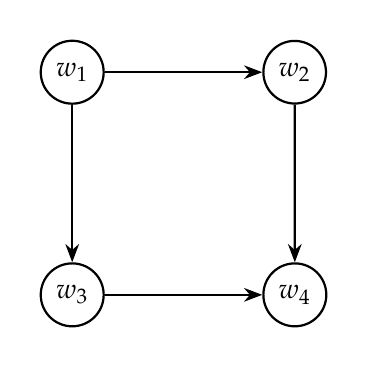
\begin{tikzpicture}[node distance=2cm,thick, >=Stealth]
\node (w1) [circle,draw] {$w_1$};
\node (w2) [circle,draw,right=of w1] {$w_2$};
\node (w3) [circle,draw,below=of w1] {$w_3$};
\node (w4) [circle,draw,right=of w3] {$w_4$};
\draw[->] (w1) -- (w2);
\draw[->] (w1) -- (w3);
\draw[->] (w2) -- (w4);
\draw[->] (w3) -- (w4);
\node [above left=1pt of w1] {};
\node [above right=1pt of w2] {};
\node [below left=1pt of w3] {};
\node [below right=1pt of w4] {};
\end{tikzpicture}
\end{document}
\caption{框架语义的示例} \label{fig:frame-validity}
\end{figure}

我们问,对于这个框架,下面的公式是否有效?
\[\Box (p\to\Box p).\]
为此,我们需要考虑四个可能世界上的情况。同样,我们只对$w_1$进行讨论,其他情况类似。对于$w_1$,有两个后继节点$w_2$,$w_3$,我们需要验证$p\to\Box p$在这两个节点上是否成立。

先考虑$w_2$,假设$p$在$w_2$上为真,我们需要验证$\Box p$是否成立。$w_2$的后继节点只有$w_4$,但我们可以让$p$在$w_4$上为假,这样$\Box p$就不成立。因此,$w_2$上$p\to\Box p$也不成立,从而$w_1$上$\Box (p\to\Box p)$不成立。

于是,我们找到了一种赋值的方案,使得$\Box (p\to\Box p)$在$w_1$上不成立。因此,这个公式在整个框架上也不有效。
\end{example}


最后,我们说明,上面的讨论在知识逻辑中都是自然成立的。此时,模态公式$K_i\phi$被读作“$i$知道$\phi$”。从语义来说,$K_i$是$\Box$算子,即我知道$\phi$意味着在我认为的所有可能世界中$\phi$都是真的,即:
\[
\mathcal M,w\vDash K_i\phi\Longleftrightarrow\text{对任意$v$,如果$w\to_i v$,那么$\mathcal M,v\vDash\phi$}。
\]
同样,模态公式的真值有两个层面:
\begin{itemize}
\item 在点模型上可满足:$\mathcal M,w\vDash\phi$;
\item 在框架上有效:$\mathcal F\vDash\phi$。
\end{itemize}

\section{模态可定义性}


\begin{frame}{模态可定义性}
\begin{itemize}
    \item 逻辑的意义在于把对事物的抽象认知用形式化的语言表述出来.
    \item 我们已经看到,我们对事物的认知可以被两种方式描述出来:
    \begin{itemize}
        \item Kripke模型(框架)的特殊结构.
        \item 具体的模态公式.
    \end{itemize}
    \item 这两种方式之间有什么联系?
\end{itemize}
\end{frame}

\begin{frame}{例子}
\begin{itemize}
    \item 考虑只有一个认知算子$K$.
    \item 如果$p$是真的,那么我不知道非$p$:$\phi:p\to\neg K\neg p$.
    \item 我们可以将对于$K$的理解反映到Kripke模型中.
    \item 真实世界是我能够感知到的可能世界:$xRx$,这是一个自反关系.
    \item 对于自反点模型以及框架,$\mathcal M,v\vDash \phi$以及$\mathcal F\vDash \phi$.
\end{itemize}
\end{frame}

\begin{frame}{例子}
\begin{itemize}
    \item $\mathcal M,w\vDash\Diamond\top$.
    \begin{itemize}
        \item 存在一个$v$,$w\to v$并且$\mathcal M,v\vDash\top$,也就是$w$有一个后继.
    \end{itemize}
    \item $\mathcal F\vDash\Diamond \top$.
    \begin{itemize}
        \item 每个基于$\mathcal F$的点模型$\mathcal M,v$都有$\Diamond \top$,即$\mathcal F$每个点都有后继.
    \end{itemize}
    \item $\mathcal F\vDash p\to\Diamond p$.
    \begin{itemize}
        \item 任意赋值$V$和任意点$w$,都有$\mathcal M,w\vDash p\to\Diamond p$.
        \item 因此,如果$w$上有$p$,那么$w$必须有一个后继上面也有$p$.
        \item  取$V$使得只有$w$上有$p$,因为对任意赋值都要成立,所以在这个赋值下,$w$必须要以自己为后继.
        \item 因此$\mathcal F$充分必要地是一个自反框架.
    \end{itemize}
\end{itemize}
\end{frame}

\begin{frame}{模态可定义性}
\begin{itemize}
    \item 从点模型的角度,我们可以讨论模态公式定义了什么样的点模型.
    \item 设$\mathcal K$是一些点模型的集合,$\Sigma$是一些模态公式的集合.
    \item 我们说$\mathcal K$可由公式集$\Sigma$定义,指的是对任意点模型$\mathcal M,w$,$\mathcal M,w\in K$当且仅当任何$\Sigma$中的公式在$\mathcal M,w$都是可满足的.
    \item 如果$\Sigma=\{\phi\}$,我们就说$K$可以由公式$\phi$定义.
    \item 对于框架可定义性,我们有类似的定义.
\end{itemize}
\end{frame}

\section{知识逻辑的基本模型与性质}\label{sec:epistemic-logic-basic-model}

\subsection{知识逻辑的Kripke模型与公理}

\subsection{Kripke模型与Aumann结构}

\subsection{“泥泞的孩童”再回顾:形式化解法}


\begin{frame}{Kripke模型的限制}
\begin{itemize}
    \item 模态算子$K_i$有特殊的性质,这要求我们对$K_i$对应的关系$R_i$也有额外的要求.
    \item 我们要求每一个$R_i$都是等价关系$\sim_i$:
    \begin{itemize}
        \item 自反:$\forall x\, x\sim_ix$.
        \item 传递:$\forall x,y,z(x\sim_iy\wedge y\sim_iz)\to x\sim_iz$.
        \item 对称:$\forall x,y(x \sim_i y\leftrightarrow y\sim_ix)$.
    \end{itemize}
    \item 从可能世界的角度来说,这一要求就是说对$i$来说,她所认为可能的世界之间都是不可区分的.
    \item 这一定义与Aumann结构的信息集是一致的.
\end{itemize}
\end{frame}
\begin{frame}{算子$K_i$的公理}
\begin{itemize}
    \item 从模态可定义性的角度来说,$R_i$的特殊性质会对应$K_i$特殊的公式.
    \item 这些公式就可以被看成关于“知道”的公理(模式)或推导规则.
    \item 承认某一条公理(模式)或推导规则就必须承认可能世界具有某一种性质,反之亦然.
\end{itemize}
\end{frame}
\begin{frame}{分配公理}
\begin{itemize}
    \item \emph{分配公理}(distribution axiom):$\vDash (K_i(\phi\to\psi)\wedge K_i\phi)\to K_i\psi$.
    \item 有效性验证.
    \begin{itemize}
        \item 假设$\mathcal M,w\vDash K_i(\phi\to\psi)$且$\mathcal M,w\vDash K_i \phi$.
        \item 于是,对所有$R_i$后继$v$都有$\mathcal M,v\vDash\phi\to\psi$和$\mathcal M,v\vDash\phi$,因而$\mathcal M,v\vDash\psi$.
        \item 根据定义,$\mathcal M,w\vDash K_i\psi$,因而对所有$\mathcal F$,分配公理有效.
    \end{itemize}
    \item 分配公理意味着拥有知识的个体可以对自己的知识做任意的演绎推理,因而假设个体是\emph{逻辑全知的}(logically omniscient).
\end{itemize}
\end{frame}
\begin{frame}{知识泛化规则}
\begin{itemize}
    \item \emph{知识泛化规则}(knowledge generalization rule):对所有$\mathcal F$,如果$\mathcal F\vDash\phi$,那么$\mathcal F\vDash K_i\phi$.
    \item 有效性验证.
    \begin{itemize}
        \item 假设$\mathcal F\vDash\phi$,这意味着对所有基于$\mathcal F$的点模型都有$\mathcal M,w\vDash\phi$.
        \item 因此,对任意$w$的$R_i$后继$v$,也有$\mathcal M,v\vDash\phi$.
        \item 所以也有$\mathcal M,w\vDash K_i\phi$成立,因而$\mathcal F\vDash K_i\phi$.
    \end{itemize}
    \item 类比:一阶逻辑推理的泛化规则.
    \item 前提成立的$\phi$是关于$\mathcal F$本身的性质(特别是关于知识),因此知识泛化规则意味着个体知道关于知识的一切性质.
    \begin{itemize}
        \item 其实更重要的是,知识的一切性质都是共同知识(练习).% HW
    \end{itemize}
\end{itemize}
\end{frame}

\begin{frame}{知识公理}
\begin{itemize}
    \item \emph{知识公理}(knowledge axiom)或\emph{真理公理}(truth axiom):$\vDash_H K_i\phi\to\phi$.
    \item 验证留作练习. % HW
\end{itemize}
\end{frame}
\begin{frame}{内省公理}
\begin{itemize}
    \item \emph{正内省公理}(positive introspective axiom):$\vDash_H K_i\phi\to K_iK_i\phi$.
    \item \emph{负内省公理}(positive introspective axiom):$\vDash_H \neg K_i\phi\to K_i\neg K_i\phi$.
    \item 验证留作练习. % HW
\end{itemize}
\end{frame}
\begin{frame}{其他公理}
\begin{itemize}
    \item 以上五条性质(四条公理+一条推导规则)加上MP形成的推理系统称为S5公理系统.
    \begin{itemize}
        \item 需要注意的是,这些公理其实都是公理模式,包含了无穷条公理.
    \end{itemize}
    \item 此外,从哲学的角度讨论,还有一些别的公理.
    \item \emph{一致性公理}(consistency axiom):$\vDash_H\neg K_i\bot$.
    \begin{itemize}
        \item 因此,个体不能够知道假的陈述,以此区别于信念.
    \end{itemize}
\end{itemize}
\end{frame}
\begin{frame}{公理与模型结构}
\begin{itemize}
    \item 我们基于框架类$H$给出了关于知识的公理.
    \item 反过来,公理对应什么样的框架结构呢?
    \item 我们总结如下表:
    \begin{table}[ht]
        \centering
       \begin{tabular}{cc}
\toprule 公理 &  $R_i$的性质 \\
\midrule $K_i \varphi \to \varphi$ & 自反性 \\
$K_i \varphi \to K_i K_i \varphi$ & 传递性 \\
$\neg K_i \varphi \to K_i \neg K_i \varphi$ & 欧氏性 \\
$\neg K_i\bot$  & 序列性\\
$\varphi \to K_i \neg K_i \neg \varphi$ & 对称性 \\
\bottomrule
\end{tabular}
    \end{table}
\end{itemize}
\end{frame}

\begin{frame}{公理与模型结构}
\begin{itemize}
    \item 欧氏性:$\forall x,y,z(xR_iy\wedge xR_iz\to yR_iz)$.
    \begin{itemize}
        \item 关系一定形成三角形.
    \end{itemize}
    \item 序列性:$\forall x\exists y\, xR_iy$.
    \begin{itemize}
        \item 所有点都有后继.
    \end{itemize}
    \item 以上验证都留作习题. % HW   
    \item 思考:从可能世界角度,$R_i$的这些性质有什么直观的含义?
    \item 思考:为什么有些公理没有对应的结构性质?(提示:注意观察一个公理/规则是否有$H$出现)
\end{itemize}
\end{frame}

\begin{frame}{公理与模型结构}
\begin{itemize}
    \item 可以看出来,以上关系其实并不是孤立的,我们有:
\begin{lemma} %HW
\begin{itemize}
    \item 如果$R_i$是自反和欧氏的,那么$R_i$是对称和传递的.
    \item 如果$R_i$是对称和传递的,那么$R_i$是欧氏的.
    \item 以下命题等价:
    \begin{itemize}
        \item $R_i$是自反、对称和传递的.
\item  $R_i$是对称、传递和序列的.
\item $R_i$是自反和欧氏的.
    \end{itemize}
\end{itemize}
\end{lemma}
\item 证明留作练习.
\end{itemize}
\end{frame}

\begin{frame}{引入共同知识算子}
\begin{itemize}
    \item 下面我们将认知逻辑语言加入共同知识算子和它的语义.
    \item 首先加入“所有人都知道”这个算子:$E\phi\leftrightarrow\bigwedge_i K_i\phi$.
    \item 记$E^k\phi$为$\underbrace{E\dots E}_k\phi$.
    \item 于是,共同知识算子$C$的语义定义为:
    \[\mathcal M,w\vDash C\phi\iff\mathcal M,w\vDash E^k\phi,\quad k=1,2,\dots\]
\end{itemize}
\end{frame}

\begin{frame}{模型含义}
\begin{itemize}
    \item 我们可以从图结构来理解共同知识算子.
    \item $\mathcal M,w\vDash E^k\phi$的含义是,从$w$出发走$k$步可到达的可能世界$v$上都有$\mathcal M,v\vDash \phi$.
    \item $\mathcal M,w\vDash C\phi$的含义则是,从$w$出发可到达的可能世界$v$上都有$\mathcal M,v\vDash \phi$.
\end{itemize}
\end{frame}

\begin{frame}{共同知识的公理}
\begin{itemize}
    \item 类似算子$K_i$,$C$也有它对应的公理和推导规则.
    \item \emph{不动点公理}(fixed-point axiom):$\vDash C\phi\leftrightarrow E(\phi\wedge C\phi)$.
    \begin{itemize}
        \item 共同知识是一个递归方程的(最小)解,这是一种不动点的视角.
    \end{itemize}
    \item \emph{归纳规则}(induction rule):如果$\mathcal F\vDash \phi\to E(\phi\wedge\psi)$,那么$\mathcal  F\vDash \phi\to C\psi$.
    \begin{itemize}
        \item 每个人都可以从真实中得到的知识,一定是共同知识.
    \end{itemize}
    \item 将S5公理系统中加入关于$E$和$C$的公理,我们就扩展了认知逻辑. 
    \item 因为$E$和$C$是用$K_i$定义的,因此他们本身并不会带来Kripke模型新的结构性质.
\end{itemize}
\end{frame}



\begin{frame}{Kripke模型与Aumann结构的关系}
\begin{itemize}
    \item 我们再一次看到逻辑和集合的对应,我们总结如下表:
    \begin{table}[ht]
        \centering
        \begin{tabular}{cc}
        \toprule
             Kripke模型&Aumann结构  \\\midrule
             可能世界&样本点\\
             公式&事件\\
             原子命题&基本事件\\
             模态算子&集合-集合映射\\
             $i$的等价关系$R_i$&$i$的划分\\
             逻辑连接词&集合操作\\\bottomrule
        \end{tabular}
    \end{table}
    \item 实际上,在S5公理系统下,这种对应可以被严格叙述并证明,我们将它留做习题. 
\end{itemize}
\end{frame}

\begin{frame}{Kripke模型与Aumann结构的关系}
\begin{itemize}
    \item Kripke语义偏好逻辑,Aumann结构偏好(Bayes)概率论,因此用数学来研究知识论就有了两种风格,一种是计算机、逻辑、哲学的风格,另一种是经济学、信息论的风格.
    \item 但是,这两种对应关系完全取决于我们对知识的那些基本假设(S5公理),所以如果这些假设被打破,那么这样的对应关系就不再成立!
    \item 例如,如果我们拿掉负自省公理,那么Kripke模型就不再是等价关系,因此不再能够对应Aumann结构的信息集.
\end{itemize}
\end{frame}

\begin{frame}{“泥泞的孩童”再回顾}
\begin{itemize}
    \item 现在,我们可以形式化、严格讨论“泥泞的孩童”这一谜题了.
    \item 这一问题对应的逻辑语言是认知逻辑语言.
    \item 可能世界是$\{0,1\}^n$的元素$x=(x_1,\dots,x_n)$,$x_i=1$表示孩子
    $i$脸上有泥巴,$x_i=0$表示$i$脸上没有泥巴.
    \item 假设每个孩童$i$对应的$R_i$都是一个等价关系.
    \item 当我们如此假设时,每个孩子唯一不是共同知识的事情就是脸上泥巴的状态,其他的所有事情都被隐含在了共同知识之中.
\end{itemize}
\end{frame}

\begin{frame}{“泥泞的孩童”再回顾}
\begin{itemize}
    \item 原子命题$p_i$:孩子$i$脸上有泥巴,$p$:至少有一个孩子脸上有泥巴.
    \item 假设现在父亲还没有说出$p$.
    \item 对于孩子$i$,他的认知中只有两个可能世界:我的脸上有泥巴,或者我的脸上没有泥巴,其他对他来说都是确定的.
    \begin{itemize}
        \item $x R_i y$当且仅当$x_j=y_j$对任意$j\neq i$成立.
    \end{itemize}
    \item 因此,框架$\mathcal F$会对应一个$n$维超立方体.
\end{itemize}
\end{frame}

\begin{frame}{“泥泞的孩童”再回顾}
\begin{itemize}
    \item $n=3$的例子:
\end{itemize}
\begin{figure}
    \centering
    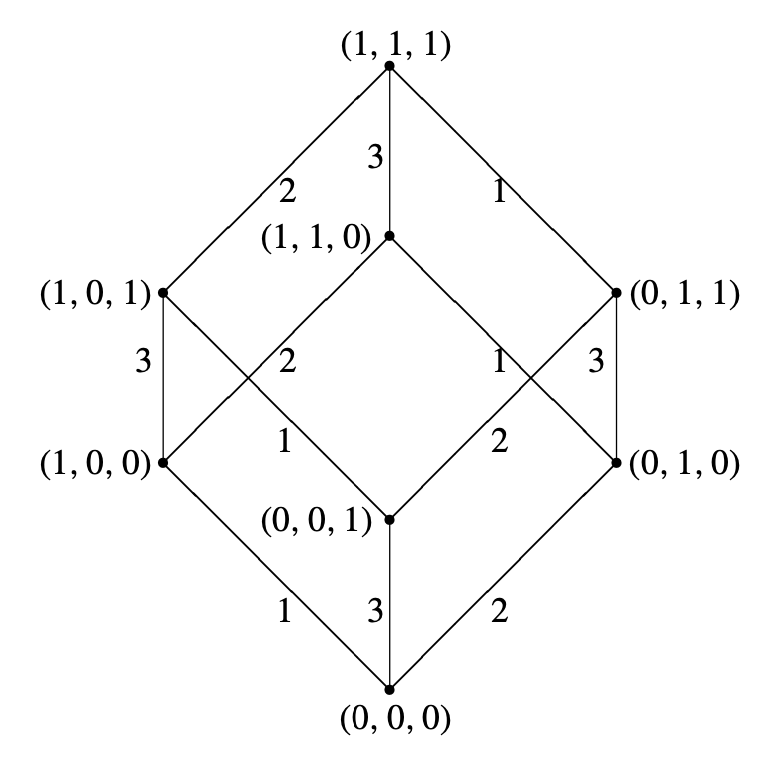
\includegraphics[scale=0.4]{Figures/modal-logic/cubic-example.png}
\end{figure}
\end{frame}

\begin{frame}{“泥泞的孩童”再回顾}
\begin{itemize}
    \item 从框架$\mathcal F$到模型$\mathcal M$,我们还需要确定赋值$V$.
    \item $w\in V(p_i)$当且仅当$w_i=1$.
    \item $w\in V(p)$当且仅当所有分量$w_j$不全为零.
    \item 从模型到点模型,我们还需要确定我们所处的可能世界,于是我们就可以讨论模态公式的可满足性.
    \item 例如:$\mathcal M,(1,0,1)\vDash Ep$,但是$\mathcal M,(1,0,1)\vDash \neg E^2p$.
\end{itemize}
\end{frame}

\begin{frame}{“泥泞的孩童”再回顾}
\begin{itemize}
    \item 假设现在父亲宣布了$p$,那么$\mathcal F$将会发生变化:
\end{itemize}
\begin{figure}[ht]
    \centering
    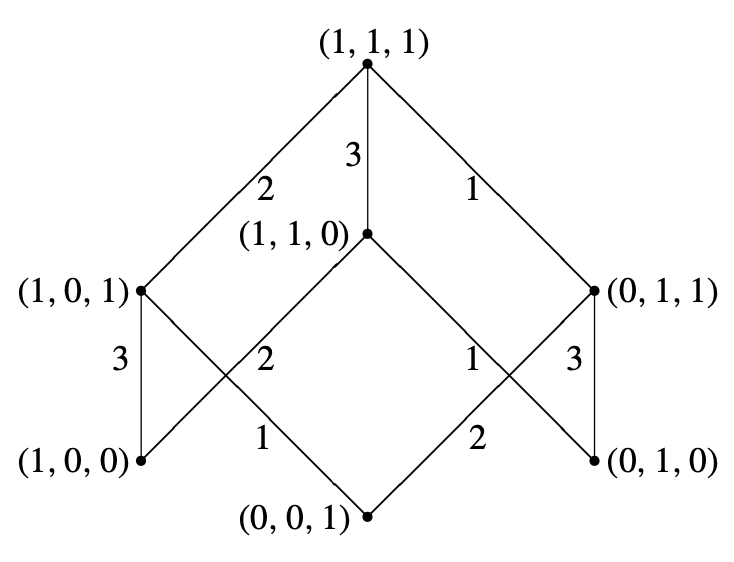
\includegraphics[scale=0.5]{Figures/modal-logic/cubic-example-after-father.png}
\end{figure}
\end{frame}

\begin{frame}{“泥泞的孩童”再回顾}
\begin{itemize}
    \item 在$i$眼中,只有两个可能世界,因此$i$回答“知道”意味着她能够确定只有一个世界;她回答不知道意味着还有两个可能世界.
    \item 假如现在是第一轮问答.
    \item 如果所有人都回答了“不知道”,考虑状态$s=(1,0,0,\dots)$.
    \item 如果真实世界是$s$,那么对于$1$来说,可能世界只有一个了,但是她却说“不知道”,说明真实世界不是$s$.
    \item 同理,所有那些只有一个$1$的可能世界都会被消掉.
    \item 因此,归纳可得,第$k$轮的时候,所有那些只有$k$个$1$的可能世界会被消掉. % HW:证明这个
\end{itemize}
\end{frame}

\begin{frame}{“泥泞的孩童”再回顾}
\begin{itemize}
    \item 如果父亲没有宣布$p$,那么$\mathcal M$是一个超立方体.
    \item 无论在任何轮,每一个孩子都会觉得两个可能世界,因此不会有任何可能世界被消掉!
    \item 因此,从结构上来说,父亲宣布$p$改变了每个孩子对应的$R_i$等价的可能世界,使得一些孩子可以确定自己所处的世界.
    \item 这一套方法可以将类似的智力谜题都用算法化的方式得到解答.
\end{itemize}
\end{frame}

\section{对不一致达成一致}

\begin{frame}{问题背景}
\begin{itemize}
    \item 本部分将用模态逻辑的方式来探讨达成一致与共同知识的关系.
    \item 最早由Aumann给出.
    \item 我们将要证明,对于有相同决策方式的两个个体来说,他们不可能对采取不同行动这件事具有共同知识.
    \item 典型故事:同样的AI之间会发生交易吗?
    \item 交易发生意味着买家和卖家有不一样的决策(一个买一个卖).
    \item 因此,如果两个人按照相同的规则来行事,那么不会有交易发生!
\end{itemize}
\begin{center}
    players cannot ``agree to disagree''.
\end{center}
\end{frame}

\begin{frame}{模型}
\begin{itemize}
    \item 假想一个含时的系统,有两个玩家1和2.
    \item 在任意时刻,每个玩家处于一个状态$s_i$之中.
    \item 每个玩家分别有一个自己的局部状态空间$S_i$.
    \item 整个系统的全局状态是$(s_1,s_2)\in S_1\times S_2=\mathcal G$.
    \item 时刻是离散的,用非负整数$m$表示,初始时刻是$0$.
    \item 系统的一次\emph{运行}(run)指的是函数$r:m\mapsto(s_1,s_2)$.
    \begin{itemize}
        \item 运行描述了系统每一时刻的全局状态.
    \end{itemize}
    \item \emph{系统}(system)$\mathcal R$指的是$\mathcal G$上所有可能运行的集合.
    \item 给定$r\in\mathcal R$,$(r,m)$被称为系统$\mathcal R$的一个点.
\end{itemize}
\end{frame}

\begin{frame}{模型}
\begin{itemize}
    \item 玩家处于某个状态的时候可以采取某种行动.
    \item 为了反映“玩家按照相同的规则行事”这件事,我们规定两个玩家的行动集都是$A$,并且这一集合不依赖于全局或局部的状态.
    \item 给定所有人的行动和一个全局状态,我们可以定义系统的\emph{转移函数}(transition function)为$\tau:A^2\times\mathcal G\to\mathcal G$.
    \begin{itemize}
        \item 因此,转移函数描述了所有人的行动如何导致系统从一个状态到另一个状态.
    \end{itemize}
\end{itemize}
\end{frame}

\begin{frame}{模型}
\begin{itemize}
    \item 如何描述“按照规则行事”?
    \item 我们用\emph{策略}来描述这种概念.
    \item 玩家$i$的策略$P_i$是一个从局部状态$S_i$到行动集$A$的映射.
    \begin{itemize}
        \item 处于什么状态就做什么事.
    \end{itemize}
    \item 两个玩家的联合策略记为$P=(P_1,P_2)$.
    \item 以上定义是Markov博弈的限制:我们要求玩家的策略只依赖于状态,但是我们也不允许玩家的行动是随机的. 
\end{itemize}
\end{frame}

\begin{frame}{模型}
\begin{itemize}
    \item 一个联合策略要执行起来,还需要初始状态.
    \item 初始状态可能的集合记为$\mathcal G_0$.
    \item 给定初始状态集$\mathcal G_0$和转移函数$\tau$,我们就可以在系统上执行任何一种策略.
    \item 我们把元组$\gamma=(\mathcal G_0,\tau)$称为系统的\emph{上下文}(context).
\end{itemize}
\end{frame}


\begin{frame}{模型}
\begin{itemize}
    \item 给定上下文$\gamma=(\mathcal G_0,\tau)$和一个联合策略$P$,我们可以讨论$P$产生的所有可能运行.
    \item 一个运行$r$与$P$\emph{相容}(compatible)指的是
    \begin{itemize}
        \item $r(0)\in\mathcal G_0$.
        \item 对任意时刻$m$,如果$r(m)=(s_1,s_2)$,那么$r(m+1)=\tau(P(s_1),P(s_2))(s_1,s_2)$.
    \end{itemize}
    \item 换言之,$r$是从跟某个可能的初始状态开始执行策略产生的运行.
    \item 一个系统$\mathcal R$表示了上下文$\gamma$和联合策略$P$,指的是所有$r\in\mathcal R$都与$P$相容. 这样的系统我们用记号$\mathcal R^{rep}(P,\gamma)$来表示.
\end{itemize}
\end{frame}



\begin{frame}{模型}
\begin{itemize}
    \item 接下来我们引入Kripke模型.
    \item Kripke模型的点是系统的点.
    \item 设原子命题集$\mathbf P$,它的元素是$perf_i(a)$,表示玩家$i$采取行动$a$.
    \item 接下来我们定义赋值函数$V$.
    \item 从$\mathbf P$的定义来看,赋值应该只依赖状态,而不依赖时间,所以我们赋值函数实际上需要分两步来定义:
    \begin{itemize}
        \item 定义$V$为从$\mathbf P$到全局状态集合的映射,
        \item 然后再扩展为到系统点集合的映射:$(r,m)\in V(p)\iff r(m)\in V(p)$.
    \end{itemize}
    \item 第一步定义如下:状态$s\in V(perf_i(a))$当且仅当在状态$s$玩家$i$采取过行动$a$.
\end{itemize}
\end{frame}

\begin{frame}{模型}
\begin{itemize}
    \item 然后我们引入知识算子$K_i$的语义.
    \item 同样,我们假设$K_i$对应的是等价关系$\sim_i$.
    \item 玩家$i$只能区分自己的局部状态$s_i$,他执行策略时,只有状态,没有时间的概念.
    \item 因此我们定义$(r,m)\sim_i (r',m')\iff r(m)_i=r'(m')_i$.
    \item 从Aumann结构来说,每一个局部状态$s_i$对应了一个信息集
    \[IS_i(s_i,\mathcal R)=\{(r,m):r\in\mathcal R,r(m)=s_i\}.\]
    \item 这样,我们就得到了Kripke点模型$\mathcal M,(r,m)$.
    \item $K_i$的语义按照基本认知逻辑定义即可.
\end{itemize}
\end{frame}

\begin{frame}{模型}
\begin{itemize}
    \item 接下来,我们引入关于时间的模态算子.
    \item 特别地,我们只引入算子$X$,表示“下一时刻”.
    \item 它的语义定义为
    \[\mathcal M,(r,m)\vDash X\phi\iff\mathcal M,(r,m+1)\vDash\phi.\]
    \item 有了算子$X$,我们可以用公式表达“将要采取行动”:
    \[act_i(a)=\neg perf_i(a)\wedge X perf_i(a).\]
\end{itemize}
\end{frame}


\begin{frame}{模型}
\begin{itemize}
    \item 接下来,我们定义关于Kripke模型的\emph{决策函数}(decision function),用它来在点模型的角度讨论策略的执行.
    \item 设Kripke模型的点集为$S$.
    \item 玩家$i$的决策函数$D$是从$S$的某些子集到行动集$A$的映射.
    \begin{itemize}
        \item 我们没有写决策函数的下标,表明两个玩家采取了相同的决策策略.
    \end{itemize}
    \item 决策函数描述的是:知道什么样的信息,就采取什么样的行动.
    \begin{itemize}
        \item 回忆Aumann结构,$S$的子集是事件.
    \end{itemize}
\end{itemize}
\end{frame}

\begin{frame}{模型}
\begin{itemize}
    \item 我们要求策略$P_i$和决策函数$D$是相容的,也就是决策函数在某个信息集上采取的行动恰好是这个策略在该状态要执行的行动:
    \[P_i(s_i)=D(IS_i(s_i,\mathcal R)),\forall s_i\in S_i.\]
    \item 反过来说,联合策略$P$在上下文$\gamma$中\emph{实现}(implement)了决策函数$D$,如果对所有$i$,$P_i$与$D$在系统$\mathcal R^{rep}(P,\gamma)$中是相容的.
\end{itemize}
\end{frame}

\begin{frame}{模型}
\begin{itemize}
    \item 策略和决策函数是两个非常容易混淆的概念,尽管他们有密切联系.
    \item 直观来说,策略就是处于什么局部状态采取什么行动,这并不涉及知识的内容.
    \item 而决策函数指的是,知道什么信息就采取什么行动,这完全是知识的内容.
    \item 在我们的背景下,
    \[\text{知道的信息}=\text{处于的局部状态}.\]
    \item 因此二者其实是从不同角度描述同一个概念.
\end{itemize}
\end{frame}

\begin{frame}{模型}
\begin{itemize}
    \item 我们对决策函数$D$有一个额外的技术要求,我们要求$D$是并-一致的(union-consistent).
    \item 具体来说,给定$S$一列互不相交的子集$T_1,\dots,T_k$,每一个都有$D(T_i)=a$,那么我们要求$D(\cup_i T_i)=a$.
    \begin{itemize}
        \item 假设我的决策函数是这样描述的:如果今天下雨,并且今天星期四,那么我会去KFC疯狂星期四;如果今天不下雨,并且今天星期四,那么我会去KFC疯狂星期四.
        \item 那么,我的决策还应该有:虽然我不知道今天下不下雨,但是如果今天是星期四,那么我会去KFC疯狂星期四.
    \end{itemize}
    \item 性质:任何联合策略都可以从某个并-一致的决策函数产生.
\end{itemize}
\end{frame}

\begin{frame}{模型}
\begin{itemize}
    \item 我们现在回顾一下这个模型.
    \item 两个玩家处于同一个系统中.
    \item 每个玩家可能知道不同的东西(局部状态空间不同,信息集不同).
    \item 但是他们的行动集相同、决策函数相同.
    \item 决策函数要求是并-一致的,由某个联合策略实现.
    \item 给定可能的初始状态和系统的转移函数(上下文),系统可以产生一系列可能的运行.
\end{itemize}
\end{frame}

\begin{frame}{达成一致定理}
\begin{theorem}[Aumann,达成一致定理,Agreement theorem]
给定联合策略$P$,上下文$\gamma$,由此产生Kripke框架$\mathcal F$. 设$a,b\in A$是两个不同的行动,如果在上下文$\gamma$中$P$实现了某个并-一致决策函数,那么
\[\mathcal F\vDash\neg C(act_1(a)\wedge act_2(b)).\]
\end{theorem}
\begin{itemize}
    \item 如果两个玩家选择了同样的并-一致决策函数,那么他们不可能对“我们采取不同行动”这件事形成共同知识.
    \item 他们不可能对不一致达成一致(agree to disagree).
\end{itemize}
\end{frame}

\begin{frame}{达成一致定理:证明}
\begin{itemize}
    \item 用反证法. 假设某个基于$\mathcal F$的点模型$\mathcal M,(r,m)$使得
    \[\mathcal M,(r,m)\vDash C(act_1(a)\wedge act_2(b)).\]
    \item 我们证明$a=b$.
    \item 思路:
    \begin{itemize}
        \item 共同知识对应了从$(r,m)$出发可到达的状态集$S'$的性质.
        \item 从玩家1的视角来看,她在$S'$所关联的信息集上都要采取行动$a$,根据并-一致性,应该有$D(S')=a$.
        \item 从玩家2来看同理,因此也应该有$D(S')=b$.
        \item 因此$a=b$.
    \end{itemize}
\end{itemize}
\end{frame}

\begin{frame}{达成一致定理:证明}
\begin{itemize}
    \item 假设$S'$是从$(r,m)$出发,通过关系$\sim_1$或$\sim_2$可到达的点集.
    \item 取一个点$(r',m')\in S'$,设$r'(m')_1=s_1'$.
    \item 假设$(r'',m'')\sim_1(r',m')$,那么$(r'',m'')\in S'$.
    \item 因此,$IS_1(s_1',\mathcal R)\subseteq S'$.
    \item 当$s_1'$取遍$S_1$,根据信息集的性质,$S'$是$IS_1(s_1',\mathcal R)$的不交并.
\end{itemize}
\end{frame}

\begin{frame}{达成一致定理:证明}
\begin{itemize}
    \item 因为$\mathcal M,(r,m)\vDash C(act_1(a))$,所以有$\mathcal M,(r',m')\vDash act_1(a)$.
    \item 这一公式意味着$P_1(s_1')=a$.
    \item 根据$P$和$D$的关系,这等价于$D(IS_1(s_1',\mathcal R))=a$.
    \item 因为这件事对任意$s_1'$都成立,根据$D$的并-一致性,$D(S')=a$.
    \item 同理,从玩家2的角度来说$D(S')=b$.
    \item 因此$a=b$.
\end{itemize}
\end{frame}

\begin{frame}{达成一致定理:拓展}
\begin{itemize}
    \item 我们的定理是对于确定性的策略证明的.
    \item 然而,一个策略可能是非确定的,也就是在一个状态可能会有多种行动的选择,比如选择带有随机性.
    \item 这个时候,达成一致定理依然成立,但是我们需要恰当地定义Kripke模型、决策函数以适应非确定性的策略.
    \item 当策略具有非确定性时,我们可以用这一模型来理解带有先验知识、风险或者不确定性下的达成一致定理.
    \begin{itemize}
        \item 只要策略能够对应一个并-一致的决策函数,结论都有效.
        \item 这实际上是Aumann最初考虑的版本,即共同信念,而不是共同知识.
    \end{itemize}
\end{itemize}
\end{frame}

\section{习题}

\section{章末注记}